\documentclass[11pt]{article}
\usepackage[T1]{fontenc}
\usepackage{lmodern}
\pdfglyphtounicode{parenleftbig}{0028}
\pdfglyphtounicode{parenrightbig}{0029}
\pdfglyphtounicode{parenleftBig}{0028}
\pdfglyphtounicode{parenrightBig}{0029}
\pdfgentounicode=1
\usepackage[margin=1.05in]{geometry}
\usepackage{amsmath,amssymb,amsthm,mathtools}
\usepackage{microtype}
\usepackage{enumitem}
\usepackage{xcolor}
\usepackage{tikz}
\usetikzlibrary{arrows.meta,positioning,calc}
\usepackage[hidelinks]{hyperref}
\hypersetup{pdftitle={A proof of Seymour's second-neighborhood conjecture},
 pdfauthor={OpenAI}, pdfsubject={Oriented graphs and finite relations}}
\pdftrailerid{}
\newtheorem{theorem}{Theorem}[section]
\newtheorem{lemma}[theorem]{Lemma}
\newtheorem{proposition}[theorem]{Proposition}
\newtheorem{corollary}[theorem]{Corollary}
\theoremstyle{remark}
\newtheorem{remark}[theorem]{Remark}
\newcommand{\abs}[1]{\lvert #1\rvert}
\DeclareMathOperator{\rank}{rank}
\DeclareMathOperator{\im}{im}
\newcommand{\R}{\mathbb R}
\newcommand{\unverified}[1]{\par\smallskip\noindent\fbox{\parbox{0.95\linewidth}{\textbf{Unverified step.} #1}}\par\smallskip}
\newcommand{\step}[1]{\par\smallskip\noindent\textbf{Step #1.}}
\newcommand{\cR}{\mathcal R}
\newcommand{\cC}{\mathcal C}
\newcommand{\cM}{\mathcal M}
\newcommand{\bu}{\mathbf u}
\newcommand{\bv}{\mathbf v}
\newcommand{\tr}{\mathsf T}
\title{A proof of Seymour's second-neighborhood conjecture}
\author{Rewritten for readability from the OpenAI manuscript of the same title}
\date{September 23, 2026}
\begin{document}
\maketitle
\begin{abstract}
We prove that every nonempty finite oriented graph has a vertex with at least
as many vertices at directed distance two as at directed distance one.
This resolves Seymour's second neighborhood conjecture positively.
The argument is presented as a sequence of individually justified steps.
\end{abstract}

\section{The result and the plan}\label{sec:introduction}

\subsection*{Statement}
An \emph{oriented graph} is a finite directed graph with no loops, no multiple
arcs, and no pair of opposite arcs; its underlying undirected graph need not be
complete or connected. We write $x\to y$ for an arc. For a vertex $v$,
\[
 N_1^+(v)=\{u:v\to u\},\qquad
 N_2^+(v)=\{w\notin\{v\}\cup N_1^+(v):v\to u\to w\text{ for some }u\}.
\]
Thus $N_2^+(v)$ is the set of vertices at directed distance exactly two from
$v$, each counted once.

\begin{theorem}\label{thm:main}
Every nonempty finite oriented graph has a vertex \(v\) such that
\(\abs{N_1^+(v)}\leq\abs{N_2^+(v)}\).
\end{theorem}

There is no connectivity or degree hypothesis; a sink ($N_1^+(v)=\varnothing$)
satisfies the conclusion trivially. In a directed triangle every vertex has
$\abs{N_1^+}=\abs{N_2^+}=1$, so the inequality cannot be made strict.

\emph{Image operator.} For a digraph $D$ and $S\subseteq V(D)$ put
\[
 F_D(S)=\{y:x\to y\text{ for some }x\in S\},\qquad F_D^2(S)=F_D(F_D(S)).
\]
The set $F_D(S)$ may meet $S$. The operator is monotone and
$F_D(S\cup S')=F_D(S)\cup F_D(S')$. In an oriented graph no walk of length two
returns to its start, so $v\notin F_D^2(\{v\})$ and
$N_2^+(v)=F_D^2(\{v\})\setminus F_D(\{v\})$.

\subsection*{Context}
The conjecture was recorded by Dean and Latka~\cite{DeanLatka1995}. For
tournaments (Dean's conjecture) it was proved by Fisher~\cite{Fisher1996}
using Farkas' lemma and by Havet and Thomass\'e~\cite{HavetThomasse2000} using
median orders; extensions to tournaments missing small structures appear in
\cite{FidlerYuster2007,Ghazal2012,DaraFrancisJacobNarayanan2022,DaamouchAlMninyGhazal2025}.
Small minimum outdegree is treated in
\cite{KanekoLocke2001,SadhukhanSandeepSen2026}, approximate ratios in
\cite{ChenShenYuster2003,HuangPeng2024}, orientations of random graphs in
\cite{BotlerMouraNaia2023,EspunyDiazEtAl2025}, and a dense case in
\cite{Brukhman2026}. The present proof builds on the minimal-counterexample and
graph-product methods of Brantner, Brockman, Kay and
Snively~\cite{BrantnerBrockmanKaySnively2009} and on Seacrest's subset
perspective~\cite{Seacrest2019}; the main additional ingredient is a pruning
bound for arbitrary finite binary relations (Lemma~\ref{lem:pruning}).
Theorem~\ref{thm:main} also gives the weighted forms of the conjecture through
Seacrest's equivalences~\cite{Seacrest2015}
(Section~\ref{sec:weighted-consequences}) and consequences for short directed
cycles (Section~\ref{sec:directed-cycle-consequences}).

\subsection*{Proof at a glance}
The theorem is proved by contradiction, in three parts.
\begin{enumerate}[label=\textup{(\Alph*)},leftmargin=*]
\item \emph{Reduction} (Section~\ref{sec:reduction},
Proposition~\ref{prop:counterexample-reduction}). Take a counterexample $D$ of
minimum order and then minimum number of arcs. Deleting arcs and invoking
minimality shows $\abs{F_D^2(S)\setminus F_D(S)}<\abs{F_D(S)\setminus S}$ for
every nonempty proper $S$ (Lemma~\ref{lem:subset-deficit}). Replacing each
vertex by a large transitive tournament (Lemma~\ref{lem:blowup}) yields an
oriented graph $G$ with positive indegrees and
\begin{equation}\label{eq:overview-concavity}
 \abs{U}+\abs{F_G^2(U)}<2\abs{F_G(U)}\qquad(\varnothing\ne U\subsetneq V(G)).
\end{equation}
\item \emph{Pruning} (Section~\ref{sec:pruning}, Lemma~\ref{lem:pruning});
independent of (A) and of orientation. Two families of ordered pairs over a set
with a binary relation may ``conflict''. All conflicts can be removed by
deleting members, at a cost bounded by the size of a set $H$ plus the number of
certain points left uncovered \emph{after} deletion. Deletions correspond to
vertex covers of an auxiliary bipartite graph. By K\H{o}nig's argument it
suffices to bound a maximum matching, and this is done by a rank computation
with four matrices satisfying $NL=AB$ at generic coefficients
(Lemma~\ref{lem:kernel-support} is the linear-algebra input).
\item \emph{Contradiction} (Section~\ref{sec:incompatibility},
Proposition~\ref{prop:no-concavity}): no $G$ as in (A) exists. With $X=V(G)$,
consider pairs $(P,Q)$ of subsets of $X\times X$ containing the diagonal such
that $F_1P$ (advance the first coordinate along an arc) and $F_2Q$ (advance the
second) are disjoint. Let $M=\abs P+\abs Q$, let $d$ be the number of points in
neither image, and maximize $M+d$. Applying~\eqref{eq:overview-concavity} to
the columns of $P$ and the rows of $Q$ shows that the complements of $F_2^2Q$
and $F_1^2P$ have combined size $>M+2d$. They may conflict; pruning deletes at
most $d+d'$ members, where $d'$ counts the points uncovered afterwards, and
keeps the diagonal. The new objective exceeds $M+2d-(d+d')+d'=M+d$, a
contradiction. The cancellation of $d'$ is why the pruning cost must be charged
to points uncovered after deletion.
\end{enumerate}
Dependencies: Lemma~\ref{lem:subset-deficit} $\Rightarrow$
Lemma~\ref{lem:blowup} $\Rightarrow$
Proposition~\ref{prop:counterexample-reduction};
Lemma~\ref{lem:kernel-support} $\Rightarrow$ Lemma~\ref{lem:pruning}
$\Rightarrow$ Proposition~\ref{prop:no-concavity}; the two propositions give
Theorem~\ref{thm:main}, which gives Corollaries~\ref{cor:weighted-forms}
and~\ref{cor:directed-cycle-consequences}.

\emph{Renamed symbols.} To keep one meaning per symbol: in
Lemma~\ref{lem:subset-deficit} the lost out-neighbors form $Y$ (source: $Q$)
and the degrees are $\nu_1,\nu_2$ (source: $d_1,d_2$); in
Lemma~\ref{lem:blowup} label sets are $U_x$ (source: $T_v$); in
Section~\ref{sec:pruning} the support-rank matrices are $\Theta,\Theta^{p,i}$
with supports $\Omega,\Omega^{p,i}$ (source: $D$, $T$) and vectors are bold; in
Section~\ref{sec:weighted-consequences} we write $\mathrm{Arc}(D)$, $\omega$,
$\gamma_v^\omega$, $\Phi_D$ (source: $A(D)$, $w$, $\beta_v^w$, $M_D$); in
Section~\ref{sec:directed-cycle-consequences} we write $\overline N(v)$,
$\deg^\pm$ (source: $Z(v)$, $d^\pm$).

\section{From a counterexample to a strict subset inequality}
\label{sec:reduction}

In this section $D$ is a base oriented graph and $F=F_D$.

\begin{proposition}[Counterexample reduction]
\label{prop:counterexample-reduction}
If Theorem~\ref{thm:main} has a counterexample, then there is a finite
nonempty oriented graph $G$ in which every vertex has positive indegree
and
\begin{equation}
\label{eq:strict-subset-growth}
  \abs{U}+\abs{F_G^2(U)}<2\abs{F_G(U)}
  \qquad\text{for every }\varnothing\ne U\subsetneq V(G).
\end{equation}
\end{proposition}

The proof, at the end of this section, combines Lemma~\ref{lem:subset-deficit}
(minimality gives a strict deficit for subsets) with Lemma~\ref{lem:blowup}
(a blow-up amplifies it). The proposition is used only in the proof of
Theorem~\ref{thm:main}.

The arc-deletion argument adapts the proof idea of
\cite[Lemma~4]{Seacrest2019}. With Seacrest's parameter $\lambda$ equal to $1$,
his statement gives $\abs{F^2(S)\setminus F(S)}<\abs{F(S)}$ in an edge-minimal
counterexample when $F(S)\ne\varnothing$. Lemma~\ref{lem:subset-deficit}
replaces the right-hand side by $\abs{F(S)\setminus S}$ for nonempty proper
$S$, under the stronger minimality below; it is proved in full.

\begin{lemma}[Subset deficit]
\label{lem:subset-deficit}
Let $D$ be a finite nonempty oriented graph such that
$\abs{N_1^+(v)}>\abs{N_2^+(v)}$ for every $v\in V(D)$.
Choose $D$ with minimum order and, subject to that, minimum number of
arcs among all graphs with this property. Then $D$ is strongly connected,
every vertex has positive indegree, and
\begin{equation}
\label{eq:subset-deficit}
  \abs{F^2(S)\setminus F(S)}<\abs{F(S)\setminus S}
  \qquad\text{for every }\varnothing\ne S\subsetneq V(D).
\end{equation}
\end{lemma}

\begin{proof}
\emph{Plan.} After two structural steps we fix $S$ and grow a set $T$ from
$\varnothing$ to $E=F(S)\setminus S$. Each growth step comes from deleting arcs
and invoking arc-minimality, and it increases a counting function $g$ by
strictly less than the number of vertices added. Throughout, $N_i(x)$ means
$N_i^+(x)$ computed in $D$.

\step{1 (no sink)} A sink $x$ has $\abs{N_1(x)}=0\le\abs{N_2(x)}$, against the
hypothesis. So $D$ has no sink, hence at least two vertices.

\step{2 (strong connectivity)} Suppose $D$ is not strongly connected. Then
some strong component $V_0\ne V(D)$ has no arc leaving it (a terminal component
of the acyclic condensation). For $x\in V_0$ every walk from $x$ stays in
$V_0$, so $N_1(x)$ and $N_2(x)$ are the same in the induced subgraph $D[V_0]$
as in $D$. Thus $D[V_0]$ satisfies the hypothesis and has fewer vertices,
contradicting minimum order. So $D$ is strongly connected; having at least two
vertices, each vertex has an in-neighbor.

\step{3 (set-up)} Fix $\varnothing\ne S\subsetneq V(D)$ and put
\[
  I=F(S)\cap S,\qquad E=F(S)\setminus S,
  \qquad g(T)=\abs{F(T)\setminus(I\cup T)}\quad(T\subseteq E).
\]
So $F(S)=I\sqcup E$. Strong connectivity gives an arc from $S$ to its
complement, so $E\ne\varnothing$.

\step{4 (delete arcs)} Fix $T\subsetneq E$. Let $D_T$ be $D$ with all arcs from
$S$ to $E\setminus T$ deleted; write $N_i'$, $F'$ for neighborhoods and images
in $D_T$. Every vertex of $E\setminus T\ne\varnothing$ is the head of an arc
from $S$, so $D_T$ is an oriented graph of the same order with fewer arcs. By
the choice of $D$ it fails the hypothesis: some vertex $v$ has
\begin{equation}\label{eq:DT-fails}
 \abs{N_1'(v)}\le\abs{N_2'(v)}.
\end{equation}

\step{5 ($v$ lost out-neighbors)} Let $Y=N_1(v)\setminus N_1'(v)$. If
$Y=\varnothing$, then $N_1'(v)=N_1(v)$ and $N_2'(v)\subseteq N_2(v)$ (a
two-step path in $D_T$ is one in $D$, and the excluded set $\{v\}\cup N_1(v)$
is unchanged), so $\abs{N_1(v)}\le\abs{N_2'(v)}\le\abs{N_2(v)}$, against the
hypothesis on $D$. Hence $Y\ne\varnothing$. Only arcs from $S$ into
$E\setminus T$ were deleted, so $v\in S$ and $Y=N_1(v)\cap(E\setminus T)$.
Since $N_1(v)\subseteq F(S)=I\cup T\cup(E\setminus T)$,
\begin{equation}\label{eq:lost}
 N_1(v)\subseteq I\cup T\cup Y,\qquad N_1'(v)=N_1(v)\setminus Y\subseteq I\cup T,
 \qquad Y\cap(I\cup T)=\varnothing.
\end{equation}

\step{6 (two-step endpoints in $D_T$)} We claim
\begin{equation}
\label{eq:deleted-path-endpoints}
  F'^2(\{v\})\subseteq I\cup T\cup F(T).
\end{equation}
Let $v\to u\to w$ in $D_T$. By~\eqref{eq:lost}, $u\in I\cup T$. If
$u\in I\subseteq S$, then $w\in F(S)=I\cup E$, and $w\notin E\setminus T$
because the arc $u\to w$ survived; so $w\in I\cup T$. If $u\in T$, then
$w\in F(T)$.

\step{7 (gained second out-neighbors)}
$N_2'(v)\setminus N_2(v)\subseteq Y\cap F(T)$. Indeed, let $w$ lie in the left
side. Then $w\ne v$ and $w$ ends a two-step path from $v$ in $D_T$, hence in
$D$; as $w\notin N_2(v)$, necessarily $w\in N_1(v)$. As $w\in N_2'(v)$, we have
$w\notin N_1'(v)$. So $w\in Y$. By~\eqref{eq:deleted-path-endpoints} and
$Y\cap(I\cup T)=\varnothing$, $w\in F(T)$.

\step{8 (lost second out-neighbors)} Put
\[
  C=F(Y)\setminus\bigl(I\cup T\cup Y\cup F(T)\bigr).
\]
Then $C\subseteq N_2(v)\setminus N_2'(v)$. Indeed, let $w\in C$ and pick
$y\in Y$ with $v\to y\to w$ in $D$. By~\eqref{eq:lost}, $w\notin N_1(v)$; and
$w\ne v$, since $y\to v$ would oppose $v\to y$. So $w\in N_2(v)$.
By~\eqref{eq:deleted-path-endpoints},
$w\notin F'^2(\{v\})\supseteq N_2'(v)$.

\step{9 (count)} Steps~7 and~8 give
$N_2'(v)\subseteq(N_2(v)\setminus C)\cup(Y\cap F(T))$ with $C\subseteq N_2(v)$.
Write $\nu_i=\abs{N_i(v)}$, so $\nu_2<\nu_1$. Then~\eqref{eq:DT-fails}
and~\eqref{eq:lost} yield
\begin{equation}\label{eq:count}
  \nu_1-\abs{Y}=\abs{N_1'(v)}\le\abs{N_2'(v)}\le\nu_2-\abs{C}+\abs{Y\cap F(T)}.
\end{equation}

\step{10 (increment of $g$)} Since $F(T\cup Y)=F(T)\cup F(Y)$,
\[
 F(T\cup Y)\setminus(I\cup T\cup Y)
 =\Bigl[\bigl(F(T)\setminus(I\cup T)\bigr)\setminus\bigl(Y\cap F(T)\bigr)\Bigr]\sqcup C,
\]
the bracket being the part inside $F(T)$ and $C$ the part outside. As
$Y\cap F(T)\subseteq F(T)\setminus(I\cup T)$ by~\eqref{eq:lost}, taking
cardinalities and using~\eqref{eq:count} gives
\begin{equation}
\label{eq:deficit-increment}
  g(T\cup Y)-g(T)=\abs{C}-\abs{Y\cap F(T)}\le\abs{Y}+\nu_2-\nu_1<\abs{Y}.
\end{equation}

\step{11 (iterate)} Set $T_0=\varnothing$. While $T_k\ne E$, apply Steps~4--10
with $T=T_k$ (always deleting from the original $D$, so minimality applies each
time) to get a nonempty $Y_k\subseteq E\setminus T_k$, and put
$T_{k+1}=T_k\sqcup Y_k$. The sets increase strictly inside the finite set $E$,
so $T_r=E$ for some $r\ge1$. Summing~\eqref{eq:deficit-increment} and using
$g(\varnothing)=\abs{F(\varnothing)\setminus I}=0$ gives
$g(E)<\sum_k\abs{Y_k}=\abs{E}$.

\step{12 (conclusion)} Since $F(S)=I\cup E$ and $F(I)\subseteq F(S)$ (as
$I\subseteq S$),
\[
  F^2(S)\setminus F(S)=\bigl(F(I)\cup F(E)\bigr)\setminus(I\cup E)=F(E)\setminus(I\cup E),
\]
whose cardinality is $g(E)<\abs{E}=\abs{F(S)\setminus S}$.
\end{proof}

The next lemma amplifies the integer deficit in~\eqref{eq:subset-deficit}. Its
construction is the lexicographic product of $D$ with a transitive tournament,
as in \cite[Theorem~4.3]{BrantnerBrockmanKaySnively2009}; here an estimate is
needed for every nonempty proper subset, not only for single vertices. It is
used only in the proof of Proposition~\ref{prop:counterexample-reduction}.

\begin{lemma}[Transitive-tournament blowup]
\label{lem:blowup}
Let $D$ be an oriented graph on $n\ge1$ vertices, all of positive
indegree, satisfying \eqref{eq:subset-deficit} for every nonempty proper
subset of $V(D)$. For an integer $m>n$, replace each vertex by a
transitive tournament on $m$ vertices. For every arc $v\to w$ of $D$,
put all arcs from the block at $v$ to the block at $w$, and put no other
arcs between distinct blocks. The resulting graph $G$ is oriented,
all its indegrees are positive, and it satisfies
\eqref{eq:strict-subset-growth}.
\end{lemma}

\begin{proof}
\emph{Plan.} Split $U$ by blocks. One unit of base-level deficit is worth a
whole block ($m$ vertices), while effects inside blocks cost at most one per
base vertex, at most $n<m$ in total.

\step{1 (inside a block)} Label each block by $1,\dots,m$ with arcs from
smaller to larger labels, and let $f$ be the image operator of this tournament
on label sets. For a nonempty label set $\Lambda$ we have
$f(\Lambda)=\{x:x>\min\Lambda\}$, so
$\Lambda\subseteq\{\min\Lambda\}\cup f(\Lambda)$ and
$f^2(\Lambda)\subseteq f(\Lambda)$. Hence
\begin{equation}
\label{eq:internal-block-bound}
  \abs{\Lambda}-\abs{f(\Lambda)}\le1,\qquad
  \abs{\Lambda}-2\abs{f(\Lambda)}+\abs{f^2(\Lambda)}\le\abs{\Lambda}-\abs{f(\Lambda)}\le1.
\end{equation}

\step{2 ($G$ is oriented with positive indegrees)} Call an arc of $G$
\emph{internal} if it lies in one block and \emph{external} otherwise.
Internal arcs form transitive tournaments; between two blocks all arcs point
one way, because $D$ has no opposite arcs. So $G$ is oriented. A vertex in the
block at $x$ receives arcs from the whole block at any in-neighbor of $x$.

\step{3 (decomposition)} Fix $\varnothing\ne U\subsetneq V(G)$. Let $U_x$ be
the set of labels of $U$ in the block at $x$, and
\[
  S=\{x\in V(D):U_x\ne\varnothing\}\ne\varnothing,\qquad H_0=F(S)\cup F^2(S).
\]
Thus $\abs U=\sum_{x\in S}\abs{U_x}$.

\step{4 (first image)} If $y\in F(S)$, some $x\in S$ has $x\to y$, and a vertex
of $U$ in the block at $x$ sends arcs to the whole block at $y$. If
$y\notin F(S)$, no external arc from $U$ enters the block at $y$, so $F_G(U)$
meets it exactly in $f(U_y)$ (empty if $y\notin S$). Hence
\[
  \abs{F_G(U)}=m\abs{F(S)}+\sum_{x\in S\setminus F(S)}\abs{f(U_x)}.
\]

\step{5 (second image)} Consider a two-step path starting at a vertex of $U$
in the block at $x\in S$. With two external arcs it ends in a block of
$F^2(S)$; with exactly one external arc, in either order, in a block of
$F(S)$; with none, at a label of $f^2(U_x)$ in the block at $x$. Bounding each
block of $H_0$ by $m$,
\[
  \abs{F_G^2(U)}\le m\abs{H_0}+\sum_{x\in S\setminus H_0}\abs{f^2(U_x)}.
\]

\step{6 (combine)} Steps~3--5 give
\begin{equation}
\label{eq:blowup-sharp}
\begin{aligned}
  \abs{U}-2\abs{F_G(U)}+\abs{F_G^2(U)}
  \le{}& m\bigl(\abs{H_0}-2\abs{F(S)}\bigr)+\sum_{x\in S}\abs{U_x}\\
  &-2\sum_{x\in S\setminus F(S)}\abs{f(U_x)}+\sum_{x\in S\setminus H_0}\abs{f^2(U_x)}.
\end{aligned}
\end{equation}
Since $F(S)\subseteq H_0$, the last sum may be extended to $S\setminus F(S)$;
this only adds nonnegative terms. Now bound $\abs{U_x}\le m$ for
$x\in S\cap F(S)$, and apply~\eqref{eq:internal-block-bound} with
$\Lambda=U_x$ for each $x\in S\setminus F(S)$. The right side
of~\eqref{eq:blowup-sharp} is then at most
\[
 m\bigl(\abs{H_0}-2\abs{F(S)}+\abs{S\cap F(S)}\bigr)+\abs{S\setminus F(S)}.
\]
Using $\abs{H_0}=\abs{F(S)}+\abs{F^2(S)\setminus F(S)}$,
$\abs{F(S)}-\abs{S\cap F(S)}=\abs{F(S)\setminus S}$ and
$\abs{S\setminus F(S)}\le n$,
\begin{equation}\label{eq:blowup-final}
 \abs{U}-2\abs{F_G(U)}+\abs{F_G^2(U)}
 \le m\bigl(\abs{F^2(S)\setminus F(S)}-\abs{F(S)\setminus S}\bigr)+n.
\end{equation}

\step{7 (case $S\subsetneq V(D)$)} By~\eqref{eq:subset-deficit} the bracket
in~\eqref{eq:blowup-final} is an integer $\le-1$, so the right side is at most
$-m+n<0$.

\step{8 (case $S=V(D)$)} Here~\eqref{eq:subset-deficit} is unavailable.
Positive indegrees in $D$ give $F(S)=V(D)$, so $F_G(U)=V(G)$ by Step~4;
positive indegrees in $G$ give $F_G^2(U)=F_G(V(G))=V(G)$. Hence
$\abs{U}-2\abs{F_G(U)}+\abs{F_G^2(U)}=\abs U-\abs{V(G)}<0$, as $U$ is proper.
\end{proof}

\begin{proof}[Proof of Proposition~\ref{prop:counterexample-reduction}]
Among counterexamples choose $D$ of minimum order and then minimum number of
arcs. Lemma~\ref{lem:subset-deficit} supplies positive indegrees
and~\eqref{eq:subset-deficit}; Lemma~\ref{lem:blowup} with any integer
$m>\abs{V(D)}$ supplies $G$.
\end{proof}

\section{Pruning two families of pairs}\label{sec:pruning}

This section is self-contained: $X$ is any finite set with any binary
relation. Lemma~\ref{lem:pruning} is used once, in Step~9 of the proof of
Proposition~\ref{prop:no-concavity}.

\begin{lemma}[Pruning]\label{lem:pruning}
Let $X$ be a finite set with a binary relation denoted by $\to$, and let
$\cR,\cC\subseteq X\times X$ be two families, regarded as
separate copies even when their coordinates agree. Say that
$(p,j)\in\cR$ and $(i,s)\in\cC$ \emph{conflict} if
$p\to i$ and $s\to j$. Define
\begin{align*}
 Z&=\{(i,j):\text{some }(p,j)\in\cR\text{ conflicts with some }(i,s)\in\cC\},\\
 H&=\{(p,s):\text{some }(p,j)\in\cR\text{ conflicts with some }(i,s)\in\cC\}.
\end{align*}
A point $(i,j)$ is \emph{covered} by a member $(p,j)\in\cR$ when
$p\to i$, and by a member $(i,s)\in\cC$ when $s\to j$;
these are the only ways a member covers a point.

There are subfamilies $\cR'\subseteq\cR$ and $\cC'\subseteq\cC$ with no
conflicts between them such that every initially conflict-free member is
retained and
\begin{equation}\label{eq:pruning-bound}
 \abs{\cR\setminus\cR'}+\abs{\cC\setminus\cC'}
 \leq\abs H+\abs{\{z\in Z:z\text{ is covered by no member of }\cR'\cup\cC'\}}.
\end{equation}
Deleted members of $\cR$ and of $\cC$ are counted separately.
\end{lemma}

\emph{Reading the definitions.} A member $(p,j)\in\cR$ covers the points
obtained by advancing its first coordinate along $\to$; a member
$(i,s)\in\cC$ covers those obtained by advancing its second coordinate. Two
members conflict exactly when they cover a common point $(i,j)$; $Z$ is the set
of such points and $H$ collects the opposite corners $(p,s)$.
\emph{Example:} $X=\{1,2\}$ with only $1\to2$, $\cR=\{(1,2)\}$,
$\cC=\{(2,1)\}$. These conflict, $Z=\{(2,2)\}$, $H=\{(1,1)\}$, and deleting
either member costs $1\le\abs H$.

The following fact is used in Step~9 of the proof. For finite index sets
$\mathcal I,\mathcal J$ and $\Omega\subseteq\mathcal I\times\mathcal J$, a real
matrix with rows indexed by $\mathcal I$ and columns by $\mathcal J$ is
\emph{supported on $\Omega$} if its entries outside $\Omega$ are zero (entries
in $\Omega$ may vanish).

\begin{lemma}[Kernels at maximum support rank]\label{lem:kernel-support}
Let $\Omega\subseteq\mathcal I\times\mathcal J$, where $\mathcal I$ and
$\mathcal J$ are finite. Suppose that
$\Theta:\R^{\mathcal J}\to\R^{\mathcal I}$ has maximum rank among all real
matrices supported on $\Omega$. Then, for every $\mathbf x\in\ker\Theta$, every
$\mathbf y\in\ker\Theta^{\tr}$, and every $(s,j)\in\Omega$, one has
$\mathbf x_j\mathbf y_s=0$.
\end{lemma}

\begin{proof}
Suppose $\mathbf x_j\mathbf y_s\ne0$. For real $\tau\neq0$ the matrix
$\Theta_\tau=\Theta+\tau e_se_j^{\tr}$ is supported on $\Omega$, and
$\Theta_\tau\mathbf x=\tau\mathbf x_je_s$, so $e_s\in\im\Theta_\tau$. For every
$\mathbf w\in\R^{\mathcal J}$,
$\Theta\mathbf w=\Theta_\tau\mathbf w-\tau\mathbf w_je_s\in\im\Theta_\tau$, so
$\im\Theta+\R e_s\subseteq\im\Theta_\tau$. But $\mathbf y$ annihilates
$\im\Theta$ (as $\mathbf y^{\tr}\Theta=0$) and $\mathbf y_s\ne0$, so
$e_s\notin\im\Theta$. Therefore $\rank\Theta_\tau>\rank\Theta$, contradicting
maximality.
\end{proof}

\begin{proof}[Proof of Lemma~\ref{lem:pruning}]
\emph{Plan.} Steps~1--3 build a bipartite graph $\Gamma$ and show that a small
vertex cover of $\Gamma$ yields the required deletion. Steps~4--10 prove that
every matching of $\Gamma$ has at most $\abs Z+\abs H$ edges, by encoding
matchings as matrix ranks. Step~11 converts a maximum matching into a cover of
the same size.

If there are no conflicts, retain everything; then $Z=H=\varnothing$ and the
claim is immediate. Below, vector spaces carry their coordinate bases, and an
empty minor has determinant $1$, so the rank arguments remain valid for empty
matchings or index sets.

\step{1 (the graph $\Gamma$)} Let $Z_L,Z_R$ be disjoint copies of $Z$, also
disjoint from $\cR$ and $\cC$; write $z_L,z_R$ for the copies of $z$. The
bipartite graph $\Gamma$ has sides
\[
 \mathcal V_L=\cR\sqcup Z_L,\qquad\mathcal V_R=\cC\sqcup Z_R,
\]
and three kinds of edges: (a) $rc$ for conflicting $r\in\cR$, $c\in\cC$;
(b) $rz_R$ whenever $r\in\cR$ covers $z\in Z$; (c) $z_Lc$ whenever $c\in\cC$
covers $z\in Z$. There are no edges between $Z_L$ and $Z_R$. See
Figure~\ref{fig:pruning}.

\begin{figure}[!ht]
 \centering
 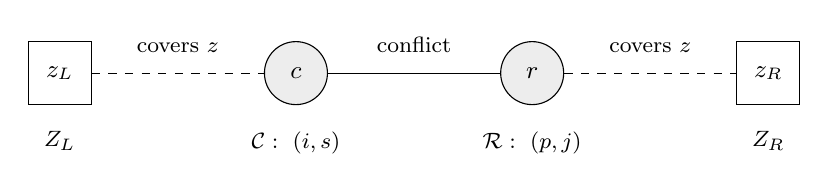
\begin{tikzpicture}[
  every node/.style={font=\small},
  original/.style={circle,draw,fill=black!7,minimum size=8mm,inner sep=1pt},
  copy/.style={rectangle,draw,minimum size=8mm,inner sep=3pt},
  edge label/.style={font=\footnotesize,above=4pt},
  family label/.style={font=\footnotesize,below=6pt}
]
 \node[copy] (zl) at (0,0) {$z_L$};
 \node[original] (c) at (3,0) {$c$};
 \node[original] (r) at (6,0) {$r$};
 \node[copy] (zr) at (9,0) {$z_R$};
 \draw[dashed] (zl) -- node[edge label] {covers $z$} (c);
 \draw (c) -- node[edge label] {conflict} (r);
 \draw[dashed] (r) -- node[edge label] {covers $z$} (zr);
 \node[family label] at (zl.south) {$Z_L$};
 \node[family label] at (c.south) {$\mathcal C:\ (i,s)$};
 \node[family label] at (r.south) {$\mathcal R:\ (p,j)$};
 \node[family label] at (zr.south) {$Z_R$};
\end{tikzpicture}
 \caption{A conflict between $r=(p,j)$ and $c=(i,s)$ forces this path, where
 $z=(i,j)\in Z$. Different conflicts can share vertices and edges.}
 \label{fig:pruning}
\end{figure}

\step{2 (conflict-free members are isolated)} Let $(p,j)\in\cR$ cover
$(i,j)\in Z$, so $p\to i$. A conflict witnessing $(i,j)\in Z$ supplies
$(i,s)\in\cC$ with $s\to j$, and this member conflicts with $(p,j)$.
Symmetrically, if $(i,s)\in\cC$ covers $(i,j)\in Z$, so $s\to j$, a witness
$(p,j)\in\cR$ with $p\to i$ conflicts with it. Hence a member with no conflict
has no edge of type (a), (b) or (c).

\step{3 (a small cover suffices)} Let $K$ be a vertex cover of $\Gamma$ with
$\abs K\le\abs Z+\abs H$ and containing no isolated vertex. Put
$\cR'=\cR\setminus K$, $\cC'=\cC\setminus K$. No conflict survives, since a
conflict is an edge and $K$ contains one of its ends. Conflict-free members are
retained by Step~2. Let $q$ be the number of points of $Z$ covered by no member
of $\cR'\cup\cC'$. Each other point $z$ is covered by some $r\in\cR'$ or
$c\in\cC'$; the edge $rz_R$ (resp.\ $z_Lc$) and $r\notin K$ (resp.\
$c\notin K$) force $z_R\in K$ (resp.\ $z_L\in K$). Distinct points give
distinct copies, so $\abs{K\cap(Z_L\sqcup Z_R)}\ge\abs Z-q$ and
\begin{equation}\label{eq:cover-charge}
 \abs{\cR\setminus\cR'}+\abs{\cC\setminus\cC'}=\abs{K\cap(\cR\sqcup\cC)}
 \leq\abs K-(\abs Z-q)\leq\abs H+q,
\end{equation}
which is~\eqref{eq:pruning-bound}. It remains to produce $K$.

\step{4 (a special maximum matching)} Among maximum matchings of $\Gamma$
choose $\cM$ with the fewest edges of type (a); let $k$ be their number. Let
$\alpha$ and $\beta$ be the sets of edges of $\cM$ of types (b) and (c), and
\[
 \ell=\abs\alpha,\qquad t=\abs\beta,\qquad\abs{\cM}=k+\ell+t.
\]
Let $\Gamma_\alpha$, $\Gamma_\beta$ be the subgraphs of $\Gamma$ induced on
$\cR\sqcup Z_R$ and on $Z_L\sqcup\cC$, and let $R_\alpha\subseteq\cR$,
$C_\beta\subseteq\cC$ be the members matched by $\alpha$, $\beta$.

\emph{Claim: $\alpha$ is a maximum matching of $\Gamma_\alpha$, and $\beta$ of
$\Gamma_\beta$.} If $\Gamma_\alpha$ had a larger matching, its symmetric
difference with $\alpha$ would contain an $\alpha$-augmenting path: a path in
$\Gamma_\alpha$ whose edges alternate outside and inside $\alpha$, with ends
$r_0\in\cR$ and $z_R\in Z_R$ unmatched by $\alpha$ and interior vertices
matched by $\alpha$. All neighbors of $z_R$ lie in $\cR$, so $z_R$ is unmatched
in $\cM$; and path edges outside $\alpha$ are outside $\cM$, since they have
type (b). If $r_0$ is unmatched in $\cM$, the path augments $\cM$,
contradicting maximality. Otherwise the $\cM$-edge $e$ at $r_0$ has type (a);
then the path augments $\cM\setminus\{e\}$, giving a matching of size
$\abs{\cM}$ with $k-1$ edges of type (a), contradicting the choice of $\cM$.
The argument for $\beta$ is the same with sides exchanged.

\step{5 (four matrices with $NL=AB$)} For each pair with $x\to y$ take real
variables $a_{xy}$ and $b_{xy}$; set $a_{xy}=b_{xy}=0$ when $x\not\to y$. For
any real assignment define linear maps
\[
 \begin{array}{ccc}
 \R^{\cR}&\xrightarrow{\ L\ }&\R^Z\\[3pt]
 {\scriptstyle B}\big\downarrow&&\big\downarrow{\scriptstyle N}\\[3pt]
 \R^H&\xrightarrow{\ A\ }&\R^{\cC}
 \end{array}
\]
by the matrix entries (row index first)
\begin{equation}\label{eq:pruning-maps}
 L_{(i,j),(p,j)}=a_{pi},\quad
 N_{(i,s),(i,j)}=b_{sj},\quad
 B_{(p,s),(p,j)}=b_{sj},\quad
 A_{(i,s),(p,s)}=a_{pi},
\end{equation}
indices ranging over the indicated sets and every entry not of a listed form
being zero. So $L,A$ move the first coordinate from $p$ to $i$, and $N,B$ move
the second coordinate from $j$ to $s$.

\emph{Claim:}
\begin{equation}\label{eq:pruning-commute}
 NL=AB.
\end{equation}
Fix a column $(p,j)\in\cR$ and a row $(i,s)\in\cC$. In $NL$ the only possible
intermediate index is $(i,j)$, and in $AB$ it is $(p,s)$; in each case the
product of the two entries is $a_{pi}b_{sj}$ if the intermediate index exists,
and the entry is $0$ otherwise. If $(p,j)$ and $(i,s)$ conflict, then
$(i,j)\in Z$ and $(p,s)\in H$, so both entries equal $a_{pi}b_{sj}$. If not,
then $p\not\to i$ or $s\not\to j$, so $a_{pi}b_{sj}=0$ and both entries vanish.

\step{6 (three rank conditions suffice)} Suppose an assignment satisfies
\[
 \rank L=\ell,\qquad\rank N=t,\qquad\dim\ker A\geq k.
\]
Then, by rank--nullity for $A$, $\im(AB)\subseteq\im A$,
and~\eqref{eq:pruning-commute},
\begin{equation}\label{eq:pruning-rank-bound}
 \abs H=\dim\ker A+\rank A\geq k+\rank(AB)=k+\rank(NL)\geq k+\ell+t-\abs Z,
\end{equation}
the last step because
$\rank(NL)=\dim\im L-\dim(\im L\cap\ker N)\geq\ell-(\abs Z-t)$. Thus
$\abs{\cM}\le\abs Z+\abs H$. Steps~7--10 produce such an assignment.

\step{7 (choice of coefficients)} We exhibit finitely many nonzero polynomials
in the variables $a_{xy},b_{xy}$ whose simultaneous nonvanishing gives what is
needed. Facts (a), (b) are instances of the correspondence between generic
matrix rank and maximum matching
size~\cite[Section~5, Theorem~1]{Edmonds1967}; we verify them directly.

\emph{(a) The matrix $L$.} The entry of $L$ at row $z=(i,j')\in Z$ and column
$r=(p,j)\in\cR$ can be nonzero only if $j'=j$ and $p\to i$, that is, only if
$rz_R$ is an edge of $\Gamma_\alpha$. A nonzero square minor of $L$ has a
nonzero term in its permutation expansion, which is a matching of
$\Gamma_\alpha$ between its columns and rows. Since $\alpha$ is maximum
(Step~4), $\rank L\le\ell$ for every assignment. Now let $L_\alpha$ be the
$\ell\times\ell$ submatrix with columns $R_\alpha$ and rows the $Z$-endpoints
of $\alpha$. Group rows and columns by the second coordinate $j$. Entries
between different groups vanish, and $\alpha$ matches within groups, so
$L_\alpha$ is block diagonal with square blocks. Inside a block, the entry at
row $(i,j)$, column $(p,j)$ is the variable $a_{pi}$ or $0$, and different
positions carry different variables. Hence different permutations contribute
different monomials to the block determinant and cannot cancel; the
permutation given by $\alpha$ contributes a nonzero monomial. So each block
determinant, and therefore $\det L_\alpha$, is a nonzero polynomial (a variable
may occur in several blocks, but a product of nonzero polynomials is nonzero).
Wherever $\det L_\alpha\neq0$: $\rank L=\ell$ and the columns of $L$ indexed by
$R_\alpha$ form a basis of $\im L$.

\emph{(b) The matrix $N^{\tr}$.} Its entry at row $(i',j)\in Z$, column
$(i,s)\in\cC$ can be nonzero only if $i'=i$ and $s\to j$, that is, along an
edge of $\Gamma_\beta$. The same argument, with blocks of fixed first
coordinate $i$ and distinct variables $b_{sj}$ inside each block, gives a
nonzero polynomial $\det(N^{\tr})_\beta$. Wherever it is nonzero,
$\rank N=\rank N^{\tr}=t$ and the columns of $N^{\tr}$ indexed by $C_\beta$
form a basis of $\im N^{\tr}$.

\emph{(c) Support ranks.} For every pair with $p\to i$ define
\[
 J_p=\{j:(p,j)\in\cR\},\quad S_i=\{s:(i,s)\in\cC\},\quad
 \Theta^{p,i}=(b_{sj})_{s\in S_i,\,j\in J_p},\quad
 \Omega^{p,i}=\{(s,j)\in S_i\times J_p:s\to j\}.
\]
For every assignment $\Theta^{p,i}$ is supported on $\Omega^{p,i}$. Let
$\rho$ be the maximum rank of real matrices supported on $\Omega^{p,i}$, and
choose such a matrix with a nonzero $\rho\times\rho$ minor (the empty minor if
$\rho=0$). The same minor of $\Theta^{p,i}$ is a polynomial $\pi^{p,i}$ in the
$b$-variables. The entries of $\Theta^{p,i}$ at positions of $\Omega^{p,i}$ are
distinct variables, so they can be assigned the entries of the chosen matrix;
thus $\pi^{p,i}$ is a nonzero polynomial. Wherever $\pi^{p,i}\ne0$,
$\Theta^{p,i}$ has rank $\rho$, the maximum among matrices supported on
$\Omega^{p,i}$.

\emph{Simultaneous choice.} The product of $\det L_\alpha$,
$\det(N^{\tr})_\beta$ and all $\pi^{p,i}$ is a nonzero real polynomial, hence
nonzero at some real assignment (induction on the number of variables). Fix
such an assignment from now on. It gives $\rank L=\ell$, $\rank N=t$, the two
basis properties, and maximum support rank for every $\Theta^{p,i}$.

\step{8 (lifts)} Let $R_0\subseteq\cR$ be the set of the $k$ left endpoints of
the type-(a) edges of $\cM$. For each such edge $rc$ ($r\in R_0$, $c\in\cC$),
the basis properties in (a), (b) give coefficients with
\begin{equation}\label{eq:pruning-lifts}
 \bu^r=e_r+\sum_{r'\in R_\alpha}\lambda_{r'}^re_{r'}\in\ker L,\qquad
 \bv^c=e_c+\sum_{c'\in C_\beta}\mu_{c'}^ce_{c'}\in\ker N^{\tr}.
\end{equation}
Since $\cM$ is a matching, $R_0\cap R_\alpha=\varnothing$ and $c\notin C_\beta$.
Hence the $r''$-coordinate of $\bu^r$ is $1$ if $r''=r$ and $0$ otherwise
($r,r''\in R_0$), and $\bv^c_c=1$.

\step{9 (kernel restriction)} \emph{Claim:} at the fixed assignment,
\begin{equation}\label{eq:conflict-kernel}
 \bu_{(p,j)}\bv_{(i,s)}=0
 \quad\text{for every conflicting }(p,j)\in\cR,\ (i,s)\in\cC
 \text{ and all }\bu\in\ker B,\ \bv\in\ker N^{\tr}.
\end{equation}
Fix such a conflict; then $p\to i$, $j\in J_p$, $s\in S_i$ and
$(s,j)\in\Omega^{p,i}$. Put $\mathbf x=(\bu_{(p,j')})_{j'\in J_p}$ and
$\mathbf y=(\bv_{(i,s')})_{s'\in S_i}$.

(i) $\Theta^{p,i}\mathbf x=0$. Take a row $s'\in S_i$. If $s'\to j'$ for some
$j'\in J_p$, then $(p,j')$ and $(i,s')$ conflict, so $(p,s')\in H$. Row
$(p,s')$ of $B$ is supported on the columns $(p,j'')$, $j''\in J_p$, so the
$(p,s')$-coordinate of $B\bu=0$ reads
\begin{equation}\label{eq:pruning-row-equation}
 \sum_{j''\in J_p}b_{s'j''}\bu_{(p,j'')}=0.
\end{equation}
If there is no such $j'$, all coefficients in~\eqref{eq:pruning-row-equation}
vanish and it holds trivially, whether or not $(p,s')\in H$.

(ii) $(\Theta^{p,i})^{\tr}\mathbf y=0$. Take a column $j'\in J_p$. If
$s'\to j'$ for some $s'\in S_i$, the resulting conflict gives $(i,j')\in Z$.
Column $(i,j')$ of $N$ is supported on the rows $(i,s'')$, $s''\in S_i$, so the
$(i,j')$-coordinate of $N^{\tr}\bv=0$ reads
\begin{equation}\label{eq:pruning-column-equation}
 \sum_{s''\in S_i}b_{s''j'}\bv_{(i,s'')}=0.
\end{equation}
Otherwise all coefficients vanish.

By Step~7(c), Lemma~\ref{lem:kernel-support} applies to $\Theta^{p,i}$ with
support $\Omega^{p,i}$ and gives $\mathbf x_j\mathbf y_s=0$, which
is~\eqref{eq:conflict-kernel}. (The perturbation inside the proof of
Lemma~\ref{lem:kernel-support} is hypothetical and concerns only
$\Theta^{p,i}$; the assignment is not changed.)

\step{10 ($\dim\ker A\ge k$)} Let $rc$ be a type-(a) edge of $\cM$; then $r,c$
conflict. Taking $\bv=\bv^c$ in~\eqref{eq:conflict-kernel} and using
$\bv^c_c=1$: every $\bu\in\ker B$ has $\bu_r=0$, for every $r\in R_0$. Now
suppose $\sum_{r\in R_0}\kappa_rB\bu^r=0$. Then
$\bu=\sum_r\kappa_r\bu^r\in\ker B$, so $\bu_r=0$ for $r\in R_0$; but
$\bu_r=\kappa_r$ by Step~8. So the $k$ vectors $B\bu^r$ are linearly
independent, and $A(B\bu^r)=NL\bu^r=0$ by~\eqref{eq:pruning-commute}
and~\eqref{eq:pruning-lifts}. Hence $\dim\ker A\ge k$. With Step~7 this gives
the three conditions of Step~6, so
\[
 \abs{\cM}=k+\ell+t\le\abs Z+\abs H.
\]

\step{11 (from the matching to a cover)} We give the matching-to-cover argument
of K\H{o}nig's theorem~\cite{konig1931}. Starting at all $\cM$-unmatched
vertices of $\mathcal V_L$, follow edges outside $\cM$ from left to right and
edges of $\cM$ from right to left; let $W_L,W_R$ be the sets of reached
vertices on the two sides. No unmatched right vertex is reached, since an
alternating path to it would augment $\cM$. The ends of an edge of $\cM$ are
both reached or both unreached: a reached right end leads to its mate, and a
matched left vertex can only be reached through its mate. Put
\[
 K=(\mathcal V_L\setminus W_L)\cup W_R.
\]
$K$ covers every edge: an edge from $W_L$ to $\mathcal V_R\setminus W_R$ can be
neither outside $\cM$ (it would be traversed) nor in $\cM$ (same reachability
of ends). $K$ contains exactly one end of each edge of $\cM$ and no unmatched
vertex (unmatched left vertices lie in $W_L$; unmatched right vertices are not
in $W_R$). So $\abs K=\abs{\cM}\le\abs Z+\abs H$, and $K$ contains no isolated
vertex. Step~3 applied to $K$ proves the lemma.
\end{proof}

\section{The extremal contradiction}\label{sec:incompatibility}

\begin{proposition}\label{prop:no-concavity}
There is no nonempty finite oriented graph $G$ in which every vertex has an
in-neighbor and whose one-step image operator
$F(U)=\{y\in V(G):x\to y\text{ for some }x\in U\}$ satisfies
\begin{equation}\label{eq:impossible-concavity}
 \abs{U}+\abs{F^2(U)}<2\abs{F(U)}
 \qquad(\varnothing\ne U\subsetneq V(G)),
\end{equation}
where $F^2=F\circ F$.
\end{proposition}

\begin{proof}
\emph{Plan.} Assume $G$ exists. Choose an extremal compatible pair $(P,Q)$
(Steps~1--2), build larger candidate families from complements of second
images (Steps~3--5), and repair them with Lemma~\ref{lem:pruning} at a cost
that the objective absorbs (Steps~6--9).

\step{1 (coordinate images)} Put $X=V(G)$. For $\Pi\subseteq X\times X$ let
\[
 F_1\Pi=\{(i,j):(p,j)\in\Pi\text{ and }p\to i\text{ for some }p\},\qquad
 F_2\Pi=\{(i,j):(i,s)\in\Pi\text{ and }s\to j\text{ for some }s\},
\]
and $F_1^2=F_1\circ F_1$, $F_2^2=F_2\circ F_2$. For fixed $j$, the column
$\Pi_j=\{p:(p,j)\in\Pi\}$ satisfies $(F_1\Pi)_j=F(\Pi_j)$ and
$(F_1^2\Pi)_j=F^2(\Pi_j)$; likewise $F_2$ acts as $F$ on each row
$\{s:(i,s)\in\Pi\}$. Let $\Delta=\{(v,v):v\in X\}$. Call $P,Q\subseteq X\times X$
\emph{compatible} if $F_1P\cap F_2Q=\varnothing$. By definition,
$(i,j)\in F_1P\cap F_2Q$ if and only if there are $(p,j)\in P$ and
$(i,s)\in Q$ with $p\to i$ and $s\to j$. So, taking the arc relation of $G$ in
Lemma~\ref{lem:pruning} with left family $P$ and right family $Q$:
compatibility means there are no conflicts, and $F_1P$ (resp.\ $F_2Q$) is the
set of points covered by members of the left (resp.\ right) family.

\step{2 (extremal pair)} The pair $(\Delta,\Delta)$ is compatible: a point
$(i,j)\in F_1\Delta\cap F_2\Delta$ would require $j\to i$ and $i\to j$. As $X$
is finite, we may choose a compatible pair with $\Delta\subseteq P\cap Q$
maximizing $M+d$, where
\[
 M=\abs{P}+\abs{Q},\qquad d=\abs{X}^2-\abs{F_1P}-\abs{F_2Q}.
\]
By compatibility, $d$ is the number of points outside $F_1P\cup F_2Q$.

\step{3 (columns of $P$ and rows of $Q$ are nonempty and proper)} The column
$P_j$ contains $j$. Suppose $P_j=X$. Positive indegrees give $F(X)=X$, so
$X\times\{j\}\subseteq F_1P$. Choose $w\to j$; then
$(w,j)\in F_2\Delta\subseteq F_2Q$, contradicting compatibility. Likewise the
row $Q_i=\{s:(i,s)\in Q\}$ contains $i$; if $Q_i=X$, then
$\{i\}\times X\subseteq F_2Q$, and choosing $w\to i$ gives
$(i,w)\in F_1\Delta\subseteq F_1P$, a contradiction.

\step{4 (summing the hypothesis)} Apply~\eqref{eq:impossible-concavity} to
$U=P_j$ and sum over $j\in X$, using Step~1; do the same for the rows of $Q$.
Since $X\ne\varnothing$,
\begin{equation}\label{eq:strict-fiber-sums}
 \abs{P}+\abs{F_1^2P}<2\abs{F_1P},\qquad\abs{Q}+\abs{F_2^2Q}<2\abs{F_2Q}.
\end{equation}

\step{5 (candidate families)} Define
\[
 \cR=(X\times X)\setminus F_2^2Q,\qquad\cC=(X\times X)\setminus F_1^2P.
\]
By~\eqref{eq:strict-fiber-sums} and the definitions of $M$ and $d$,
\begin{equation}\label{eq:complement-gain}
 \abs{\cR}+\abs{\cC}=2\abs{X}^2-\abs{F_2^2Q}-\abs{F_1^2P}
 >2\abs{X}^2+M-2\bigl(\abs{F_1P}+\abs{F_2Q}\bigr)=M+2d.
\end{equation}
These families need not be compatible.

\step{6 ($\Delta\subseteq\cR\cap\cC$)} If $(v,v)\in F_2^2Q$, there is
$s\to v$ with $(v,s)\in F_2Q$; but $(s,s)\in P$ and $s\to v$ give
$(v,s)\in F_1P$, contradicting compatibility. If $(v,v)\in F_1^2P$, there is
$p\to v$ with $(p,v)\in F_1P$; but $(p,p)\in Q$ gives $(p,v)\in F_2Q$, the same
contradiction.

\step{7 (diagonal members are conflict-free in $\cR,\cC$)} A conflict between
the left member $(v,v)$ and a right member $(i,s)\in\cC$ means $v\to i$ and
$s\to v$. From $(s,s)\in P$, advancing the first coordinate along
$s\to v\to i$ puts $(i,s)$ in $F_1^2P$, contrary to $(i,s)\in\cC$. A conflict
between a left member $(p,j)\in\cR$ and the right member $(v,v)$ means
$p\to v$ and $v\to j$. From $(p,p)\in Q$, advancing the second coordinate along
$p\to v\to j$ puts $(p,j)$ in $F_2^2Q$, contrary to $(p,j)\in\cR$.

\step{8 ($\abs H\le d$)} Let $H,Z$ be the sets attached to $\cR,\cC$ in
Lemma~\ref{lem:pruning}. We claim
\begin{equation}\label{eq:old-uncovered-bound}
 H\subseteq(X\times X)\setminus(F_1P\cup F_2Q),\qquad\text{hence}\qquad\abs{H}\le d.
\end{equation}
Fix a conflict $(p,j)\in\cR$, $(i,s)\in\cC$, $p\to i$, $s\to j$. If
$(p,s)\in F_1P$, choose $(u,s)\in P$ with $u\to p$; the path $u\to p\to i$
puts $(i,s)$ in $F_1^2P$, contrary to $(i,s)\in\cC$. If $(p,s)\in F_2Q$,
choose $(p,s')\in Q$ with $s'\to s$; the path $s'\to s\to j$ puts $(p,j)$ in
$F_2^2Q$, contrary to $(p,j)\in\cR$.

\step{9 (prune and compare)} Lemma~\ref{lem:pruning} gives conflict-free
$P'\subseteq\cR$ and $Q'\subseteq\cC$. By Steps~6--7 and its retention clause,
$\Delta\subseteq P'\cap Q'$; by Step~1, $F_1P'\cap F_2Q'=\varnothing$. So
$(P',Q')$ competes in Step~2. Put
\[
 d'=\abs{X}^2-\abs{F_1P'}-\abs{F_2Q'},
\]
the number of points outside $F_1P'\cup F_2Q'$. By Step~1 these are exactly the
points covered by no member of $P'\cup Q'$, so at most $d'$ points of $Z$ are
uncovered after pruning. By~\eqref{eq:pruning-bound}
and~\eqref{eq:old-uncovered-bound}, at most $d+d'$ members were deleted.
With~\eqref{eq:complement-gain},
\[
 \abs{P'}+\abs{Q'}+d'\ge\abs{\cR}+\abs{\cC}-(d+d')+d'>M+2d-(d+d')+d'=M+d,
\]
contradicting the maximality of $M+d$.
\end{proof}

\begin{proof}[Proof of Theorem~\ref{thm:main}]
If the theorem were false, Proposition~\ref{prop:counterexample-reduction}
would produce a nonempty finite oriented graph with positive indegrees
satisfying~\eqref{eq:impossible-concavity} for every nonempty proper vertex
set. Proposition~\ref{prop:no-concavity} rules out such a graph.
\end{proof}

\section{Weighted consequences}\label{sec:weighted-consequences}

Theorem~\ref{thm:main} yields the established weighted forms through
Seacrest's equivalences~\cite{Seacrest2015}, which concern the corresponding
assertions over all nonempty finite oriented graphs. They are not new here and
are quoted, not reproved.

\begin{corollary}[Weighted second-neighborhood forms]\label{cor:weighted-forms}
Let \(D\) be a nonempty finite oriented graph with arc set
\(\mathrm{Arc}(D)\). For a vertex weighting \(\eta:V(D)\to[0,\infty)\), write
\(\eta(S)=\sum_{x\in S}\eta(x)\). Then the following hold.
\begin{enumerate}[label=\textup{(\roman*)}]
\item For every vertex weighting \(\eta:V(D)\to[0,\infty)\), there is a
vertex \(v\) such that \(\eta(N_1^+(v))\leq\eta(N_2^+(v))\).
\item There is a vertex weighting \(\eta:V(D)\to[0,\infty)\) with
\(\sum_{x\in V(D)}\eta(x)=1\) such that
\(\eta(N_1^+(v))\leq\eta(N_2^+(v))\) for every \(v\in V(D)\).
The entries of this weighting need not all be positive.
\item For every arc weighting \(\omega:\mathrm{Arc}(D)\to[0,\infty)\), set
\(\omega(vs)=0\) when \(vs\notin\mathrm{Arc}(D)\), and for \(v,s\in V(D)\) put
\[
 \gamma_v^\omega(s)=\max\Bigl(\{0\}\cup
 \{\omega(us)-\omega(vs):u\in V(D),\ v\to u\to s\}\Bigr).
\]
Then there is a vertex \(v\) such that
\[
 \sum_{s\in V(D)}\gamma_v^\omega(s)\geq\sum_{u\in N_1^+(v)}\omega(vu).
\]
The maximum is zero if there is no indicated two-step path. Such paths are
determined by the arcs of \(D\): an arc of weight zero is still present.
\end{enumerate}
\end{corollary}

\begin{proof}
\emph{(iii).} Seacrest's Proposition~2 states that his arc-weighted
Conjecture~4 is equivalent to the unweighted conjecture, so
Theorem~\ref{thm:main} gives \textup{(iii)}.

\emph{(i).} Apply \textup{(iii)} with $\omega(us)=\eta(s)$ on every arc
$u\to s$. We claim $\gamma_v^\omega(s)=\eta(s)$ if $s\in N_2^+(v)$ and
$\gamma_v^\omega(s)=0$ otherwise. If there is no path $v\to u\to s$ (this
includes $s=v$, by orientation), the maximum is $0$. If $v\to s$, every
eligible difference is $\eta(s)-\eta(s)=0$. If $s\in N_2^+(v)$, then
$\omega(vs)=0$ and every eligible difference is $\eta(s)\ge0$. So the two sides
of \textup{(iii)} are $\eta(N_2^+(v))$ and $\eta(N_1^+(v))$. This is the
specialization noted immediately after Seacrest's Proposition~2.

\emph{(ii).} Let $\Phi_D$ be the $V(D)\times V(D)$ matrix with entry $1$ at
$(v,s)$ when $s\in N_2^+(v)$, entry $-1$ when $s\in N_1^+(v)$, and $0$
otherwise; then $(\Phi_D\eta)_v=\eta(N_2^+(v))-\eta(N_1^+(v))$. Let
$\overleftarrow D$ be $D$ with all arcs reversed. Then
$\Phi_{\overleftarrow D}=\Phi_D^{\tr}$: $s$ is an out-neighbor of $v$ in
$\overleftarrow D$ iff $v\in N_1^+(s)$ in $D$, and $s$ is an exact second
out-neighbor of $v$ in $\overleftarrow D$ iff $s\ne v$, $s\not\to v$ and
$s\to u\to v$ for some $u$ in $D$, i.e.\ iff $v\in N_2^+(s)$ in $D$. Seacrest's
Theorem~1 applies Farkas' lemma to give either a nonzero $\eta\ge0$ with
$\Phi_D\eta\ge0$, or a $\xi\ge0$ with $\Phi_D^{\tr}\xi<0$ at every coordinate.
The latter says $\xi(N_2^+(v))<\xi(N_1^+(v))$ in $\overleftarrow D$ for every
$v$, contradicting \textup{(i)} for $\overleftarrow D$. Normalizing the former
$\eta$ to total weight one proves \textup{(ii)}.
\end{proof}

\section{Directed-cycle consequences}\label{sec:directed-cycle-consequences}

In an oriented graph with no directed triangle, every exact second
out-neighbor is a non-neighbor. The first assertion below is the
oriented-graph form of Thomass\'e's non-neighbor statement recorded by
Sullivan~\cite[Conjecture~6.12]{Sullivan2006}; the consequence using both
minimum degrees is noted in \cite[Section~3]{Sullivan2006}. The regular case
gives the girth-four lower bound in the Behzad--Chartrand--Wall minimum-order
conjecture~\cite{BehzadChartrandWall1970}, also recorded
in~\cite[Section~4]{Sullivan2006}.

\begin{corollary}[Non-neighbors and directed cycles]\label{cor:directed-cycle-consequences}
Let \(D\) be a nonempty finite oriented graph of order \(n\). For
\(v\in V(D)\), write
\[
 N_1^-(v)=\{u:u\to v\},\qquad
 \deg^\pm(v)=\abs{N_1^\pm(v)},\qquad
 \delta^\pm(D)=\min_{x\in V(D)}\deg^\pm(x),
\]
and define the non-neighbors of \(v\), excluding \(v\) itself, by
\(\overline N(v)=V(D)\setminus\bigl(\{v\}\cup N_1^+(v)\cup N_1^-(v)\bigr)\).
Then the following hold.
\begin{enumerate}[label=\textup{(\roman*)}]
\item If \(D\) has no directed \(3\)-cycle, then some vertex \(v\) satisfies
\(\deg^+(v)\leq\abs{\overline N(v)}\) and
\(n-1\geq2\deg^+(v)+\deg^-(v)\).
\item If \(\delta^+(D)\geq n/3\) and \(\delta^-(D)\geq n/3\), then \(D\)
contains a directed \(3\)-cycle.
\item If \(r\geq1\) is an integer, \(\deg^+(v)=\deg^-(v)=r\) for every vertex,
and \(D\) has directed girth exactly four, then \(n\geq3r+1\).
\end{enumerate}
Here directed girth is the length of a shortest directed cycle.
\end{corollary}

\begin{proof}
\emph{(i).} Suppose \(D\) has no directed \(3\)-cycle. Let \(w\in N_2^+(v)\),
with a path \(v\to u\to w\). By definition \(w\ne v\) and
\(w\notin N_1^+(v)\); and \(w\notin N_1^-(v)\), since \(w\to v\) would close a
directed \(3\)-cycle. Thus \(N_2^+(v)\subseteq\overline N(v)\) for every
\(v\), and Theorem~\ref{thm:main} gives a vertex with
\(\deg^+(v)\leq\abs{N_2^+(v)}\leq\abs{\overline N(v)}\). Since \(D\) is
oriented, \(N_1^+(v)\) and \(N_1^-(v)\) are disjoint, so
\[
 n-1=\deg^+(v)+\deg^-(v)+\abs{\overline N(v)}\geq2\deg^+(v)+\deg^-(v).
\]

\emph{(ii).} If \(D\) had no directed \(3\)-cycle, \textup{(i)} would give
\(n-1\geq2\delta^+(D)+\delta^-(D)\geq n\), a contradiction. (No rounding is
involved, so the case \(3\mid n\) is included.)

\emph{(iii).} Directed girth four excludes directed \(3\)-cycles, and in the
regular case \textup{(i)} reads \(n-1\geq3r\).
\end{proof}

\section*{Verification checklist}

No step was left unverified in this rewrite. The load-bearing steps, in
suggested order of scrutiny:
\begin{enumerate}[leftmargin=*]
\item \textbf{Cover accounting} (Lemma~\ref{lem:pruning}, Steps~2--3): that
conflict-free members are isolated, and that a cover of size
$\le\abs Z+\abs H$ yields~\eqref{eq:pruning-bound}. This is where ``uncovered
after deletion'' enters.
\item \textbf{$NL=AB$ and the rank count} (Steps~5--6):
identity~\eqref{eq:pruning-commute} entry by entry,
then~\eqref{eq:pruning-rank-bound}.
\item \textbf{One assignment for all conditions} (Step~7): $\rank L\le\ell$
uses maximality of $\alpha$ in $\Gamma_\alpha$ (Step~4, which uses the minimal
choice of $k$); the three families of polynomials are nonzero and are made
nonzero simultaneously.
\item \textbf{Kernel restriction} (Step~9, with
Lemma~\ref{lem:kernel-support}): equations~\eqref{eq:pruning-row-equation}
and~\eqref{eq:pruning-column-equation} hold for \emph{every} row and column of
$\Theta^{p,i}$, including those whose index is absent from $H$ or $Z$. Then
Step~10 gives $\dim\ker A\ge k$.
\item \textbf{Extremal step} (Proposition~\ref{prop:no-concavity}): columns
and rows are proper (Step~3), so~\eqref{eq:impossible-concavity} applies;
diagonal members are conflict-free (Step~7); $\abs H\le d$ (Step~8); the final
arithmetic (Step~9).
\item \textbf{Arc deletion} (Lemma~\ref{lem:subset-deficit}, Steps~5--10):
inclusion~\eqref{eq:deleted-path-endpoints}, the gain and loss sets, and the
exact increment~\eqref{eq:deficit-increment}.
\item \textbf{Blow-up} (Lemma~\ref{lem:blowup}, Steps~4--8): the two image
counts, the passage to~\eqref{eq:blowup-final}, and the separate case
$S=V(D)$.
\item \textbf{External inputs.} Theorem~\ref{thm:main} uses only standard
linear algebra and augmenting paths. Section~\ref{sec:weighted-consequences}
additionally relies on the quoted statements of~\cite{Seacrest2015}, which
were not rechecked here.
\end{enumerate}

\bibliographystyle{plain}
\bibliography{references}
\end{document}
